\section{Introduction}
\label{sec:intro}

Joins are the cornerstone of relational database queries.  However, query optimizers face extreme difficulty when planning large multi-way join queries, as the search space of join orders grows exponentially as the number of relations increases.  In fact, finding the optimal join order of a query is well-known to be NP-hard in general~\cite{cluet_complexity_1995,scheufele_constructing_1996}. For this reason, beyond a small number of joins, current query optimizers must abandon exhaustive dynamic programming and resort to heuristic or greedy algorithms.  As a consequence, real-world optimizers often miss the best plans and produce suboptimal ones that can be by orders of magnitude slower.

The database theory community has long been providing tools that exploit query structures to tackle this complexity.  These approaches usually \emph{decompose} queries into specific tree structures, such as join trees~\cite{yannakakis_algorithms_1981} using the GYO algorithm~\cite{grahamGYO,DBLP:conf/compsac/YuO79}, which were later generalized to hypertree decompositions~\cite{DBLP:journals/jcss/GottlobLS02}. The resulting decompositions effectively capture the hardness of queries and, through specific requirements on connectivity, allow one to evaluate queries with theoretically-guaranteed instance-optimal complexity using the Yannakakis algorithm~\cite{bernstein_using_1981,yannakakis_algorithms_1981} or its variants~\cite{wang_yannakakis_2025,DBLP:journals/jcss/GottlobLS02}.
Over the years, these structure-based methods have been generalized to evaluate joins with projections~\cite{PODS251,PODS252,CDE}, aggregations~\cite{AJAR, FAQ}, differences~\cite{SIGMOD23, PODS24}, top-$k$~\cite{wang2023relational}, comparisons~\cite{SIGMOD22}, etc., all with strong theoretical performance guarantees.  These results suggest that leveraging a query’s structural properties can be of great help for query optimization and can dramatically improve query evaluation, with robust worst-case bounds. Yet, in practice, despite limited attempts by, e.g., Scarcello et al.~\cite{scarcello_weighted_2007}, RelationalAI~\cite{submodularwidth}, and Gottlob et al.~\cite{gottlob_reaching_2023}, real-world systems rarely utilize such structure-based approaches. Therefore, they continue to struggle with large, complex queries.

Why are structure-based methods rarely adopted in mainstream systems? A core obstacle is the dichotomy between cost-based plan search and structure-based evaluation~\cite{koutris_database_2026}. Current cost-based optimizers usually search for query plans with optimal or near-optimal cost under some cost model using
(1)~\textbf{exact algorithms}, mostly based on dynamic programming, such as~\cite{selinger_access_1979,vance_rapid_1996,vance_join-order_1998,moerkotte_dynamic_2008,stoian_dpconv_2024}, which have to run in exponential time, and thus do not scale to very large numbers of relations;
(2)~\textbf{heuristic strategies} such as greedy operator ordering (GOO)~\cite{fegaras_new_1998}, 
iterative dynamic programming~\cite{kossmann_iterative_2000}, UnionDP~\cite{mancini_efficient_2022}, and adaptive approaches~\cite{neumann_adaptive_2018,birler_optimizing_2025}, which have neither optimality guarantees nor a reasonable approximation factor unless under some assumption, such as independence of predicate selectivities;
% , of the cost function
(3)~\textbf{transformation-based techniques}, such as the Volcano/Cascades framework~\cite{graefe_volcano_1993,graefe_cascades_1995} and genetic algorithms~\cite{bennett_genetic_1991};
and
(4) more recently, \textbf{machine learning--based tuning and rewriting}~\cite{marcus_bao_2021,yang_balsa_2022,chen_efficient_2022,zhou_learned_2023,zhou_learned_2021,li_llm-r2_2024}.
Although certain approaches leverage, e.g., \emph{query graphs}~\cite{moerkotte_dynamic_2008,neumann_adaptive_2018,mancini_efficient_2022,birler_optimizing_2025}, they only show the existence of join attributes between relations but do not have a clear connection with the requirements of the aforementioned structural decompositions that help reason about asymptotic complexities.
\begin{figure}
    \centering
    \begin{subfigure}{.33\linewidth}
        \small
        \centering
        \begin{tikzpicture}[hypergraph,xscale=.7,yscale=.5,trim left=0cm,trim right=0cm]
            \node[vertex,label={east:$x_1$}] (x1) at (0, 0) {};
            \node[vertex,label={east:$x_2$}] (x2) at (-2, -2) {};
            \node[vertex,label={west:$x_3$}] (x3) at (2, -2) {};
            \node[vertex,label={east:$x_4$}] (x4) at (0, 0.75) {};
            \node[vertex,label={west:$x_5$}] (x5) at (-1, -1) {};
            \node[vertex,label={east:$x_6$}] (x6) at (1, -1) {};
            \node[vertex,label={west:$x_7$}] (x7) at (0, -2) {};
        
            \begin{scope}[on background layer]
                
                \newcommand*{\pathri}{($(x2) + (0,-0.4)$)
                    to[out=0,in=-135] ($(x5) + (-0.25,0.25)$)
                    to[out=45,in=180] ($(x1) + (0,-0.5)$)
                    to[out=0,in=135] ($(x6) + (0.25,0.25)$)
                    to[out=-45,in=180] ($(x3) + (0,-0.4)$)
                    to[out=0,in=0] ($(x4) + (0,0.5)$)
                    to[out=180,in=180] ($(x2) + (0,-0.4)$)
                }

                \newcommand*{\pathrii}{	($(x1) + (0.3,0.3)$)
                    to[out=135,in=45] ($(x5) + (-0.45,0.45)$)
                    to[out=-135,in=135] ($(x2) + (-0.3,-0.3)$)
                    to[out=-45,in=-135] ($(x5) + (0.45,-0.45)$)
                    to[out=45,in=-45] ($(x1) + (0.3,0.3)$)}
                
                \newcommand*{\pathriii}{($(x1) + (-0.3,0.3)$)
                    to[out=45,in=135] ($(x6) + (0.45,0.45)$)
                    to[out=-45,in=45] ($(x3) + (0.3,-0.3)$)
                    to[out=-135,in=-45] ($(x6) + (-0.45,-0.45)$)
                    to[out=135,in=-135] ($(x1) + (-0.3,0.3)$)}
                    
                \newcommand*{\pathriv}{	($(x2) + (0,0.4)$)
                    to[out=0,in=180] ($(x3) + (0,0.4)$)
                    to[out=0,in=90] ($(x3) + (0.5,0)$)
                    to[out=-90,in=0] ($(x3) + (0,-0.4)$)
                    to[out=180,in=0] ($(x2) + (0,-0.4)$)
                    to[out=180,in=-90] ($(x2) + (-0.5,0)$)
                    to[out=90,in=180] ($(x2) + (0,0.4)$)}
                
                \draw[hyperedge,looseness=.85, draw=BurntOrange,fill=BurntOrange,fill opacity=.1] \pathri;
                \draw[hyperedge,looseness=.85,draw=Red,fill=Red,fill opacity=.1] \pathrii;
                \draw[hyperedge,looseness=.85,draw=Fuchsia,fill=Fuchsia,fill opacity=.1] \pathriii;
                \draw[hyperedge,looseness=.85,draw=NavyBlue,fill=NavyBlue,fill opacity=.1] \pathriv;

                \node[text=BurntOrange] at (2,0.75) {$R_1$};
                \node[text=Red] at (-0.5,-1) {$R_2$};
                \node[text=Fuchsia] at (0.5,-1) {$R_3$};
                \node[text=Cyan] at (0.5,-2) {$R_4$};
                
            \end{scope}
        \end{tikzpicture}
        \caption{Query hypergraph}
        \label{fig:123-12-13-23-hg}
    \end{subfigure}
    \hfill
    \begin{subfigure}{.66\linewidth}
        \small
        \centering
        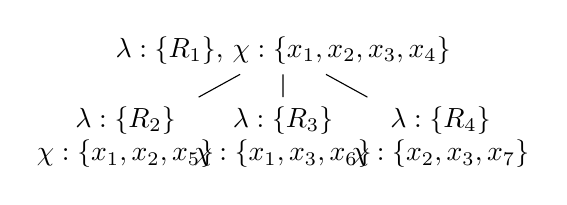
\begin{tikzpicture}[
			level distance=1.1cm,
			level 1/.style={sibling distance=2cm}
        ]
			\node { $\lambda: \{ R_1 \}$, $\chi : \{ x_1, x_2, x_3, x_4 \}$ }
				child { node[align=center] {$\lambda: \{ R_2 \}$ \\ $\chi: \{ x_1, x_2, x_5 \}$} edge from parent[-] }
                child { node[align=center] {$\lambda: \{ R_3 \}$ \\ $\chi: \{ x_1, x_3, x_6 \}$} edge from parent[-] }
                child { node[align=center] {$\lambda: \{ R_4 \}$ \\ $\chi: \{ x_2, x_3, x_7 \}$} edge from parent[-] } ;
		\end{tikzpicture}
        \caption{A join tree / hypertree decomposition}
        \label{fig:123-12-13-23-meta}
    \end{subfigure}
    \hfill\ 

    \hfill
    \begin{subfigure}{.32\linewidth}
        \centering
        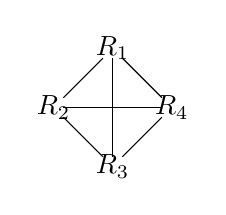
\begin{tikzpicture}[xscale=.75,yscale=.75]
            \node[label={center:$R_1$}] (R1) at (0,1) {};
            \node[label={center:$R_2$}] (R2) at (-1,0) {};
            \node[label={center:$R_3$}] (R3) at (0,-1) {};
            \node[label={center:$R_4$}] (R4) at (1,0) {};
            \draw (R1) -- (R2);
            \draw (R1) -- (R3);
            \draw (R1) -- (R4);
            \draw (R2) -- (R3);
            \draw (R2) -- (R4);
            \draw (R3) -- (R4);
        \end{tikzpicture}
        \caption{Query graph}
        \label{fig:123-12-13-23-qg}
    \end{subfigure}
    \hfill
    \begin{subfigure}{.32\linewidth}
        \centering
        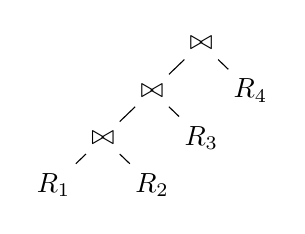
\begin{tikzpicture}[
			level distance=0.6cm,
			level 1/.style={sibling distance=1.25cm},
        ]
			\node { $\bowtie$ }
                child { node {$\bowtie$} edge from parent[-]
    				child { node {$\bowtie$} edge from parent[-]
                        child { node {$R_1$} edge from parent[-] }
                        child { node {$R_2$} edge from parent[-] }
                    }
                    child { node {$R_3$} edge from parent[-] }            
                } child { node {$R_4$} edge from parent[-] }
            ;
		\end{tikzpicture}
        \caption{A width-1 query plan}
        \label{fig:123-12-13-23-hierarchical-plan}
    \end{subfigure}
    \hfill
    \begin{subfigure}{.32\linewidth}
        \centering
        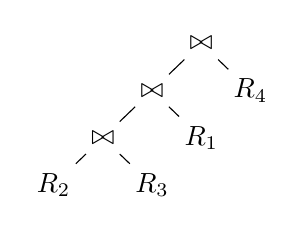
\begin{tikzpicture}[
			level distance=0.6cm,
			level 1/.style={sibling distance=1.25cm}
        ]
			\node { $\bowtie$ }
                child { node {$\bowtie$} edge from parent[-]
    				child { node {$\bowtie$} edge from parent[-]
                        child { node {$R_2$} edge from parent[-] }
                        child { node {$R_3$} edge from parent[-] }
                    }
                    child { node {$R_1$} edge from parent[-] }            
                } child { node {$R_4$} edge from parent[-] }
            ;
		\end{tikzpicture}
        \caption{A width-2 query plan}
        \label{fig:123-12-13-23-non-hierarchical-plan}
    \end{subfigure}
    \hfill\ 
    \caption{The hypergraph, a join tree, the query graph, and two query plans of the query $Q_{\ref{ex:123-12-13-23-intro}}$ in \cref{ex:123-12-13-23-intro}}
    \label{fig:123-12-13-23}
\end{figure}


\begin{example} \label{ex:123-12-13-23-intro}
    Consider the query
    \begin{align*}
        Q_{\ref{ex:123-12-13-23-intro}} \gets \pi_{\emptyset} (& R_1[x_1, x_2, x_3, x_4] \bowtie R_2[x_1, x_2, x_5] \bowtie R_3[x_1, x_3, x_6] \bowtie R_4[x_2, x_3, x_7]),
    \end{align*}
    which is a Boolean acyclic query.
    Its hypergraph is shown in \cref{fig:123-12-13-23-hg}, and a join tree, which is also a hypertree decomposition, in \cref{fig:123-12-13-23-meta}.
    Its query graph, as shown in \cref{fig:123-12-13-23-qg}, is a clique with the four relations as vertices, as each pair shares some join attribute.
    \cref{fig:123-12-13-23-hierarchical-plan} is a query plan that follows the structure of the join tree (which we formally define later). \cref{fig:123-12-13-23-non-hierarchical-plan} does not, but it is still within the search space of traditional algorithms according to the query graph.
\end{example}

Theoretical research typically focuses on worst-case asymptotic data complexity, assuming that cost differences among decompositions are negligible.  
In practice, however, different decompositions may lead to significantly different concrete cost values.
Therefore, using only structural properties, such as hypertree widths, is not sufficient~\cite{gottlob_reaching_2023}.
However, selecting the best decomposition is challenging, as there can be an exponential number of candidates. 
Without an efficient cost-based exploration of alternatives, explicitly scanning through all of them would be computationally prohibitive.
Furthermore, evaluation plans for structure-based methods are not natively supported by current systems that use standard binary query plans~\cite{koutris_database_2026,gottlob_reaching_2023}. As a result, deploying them requires a dedicated optimization and execution pipeline, which limits their practical adoption.

\subsection{Our Contributions}

In this work, we take a major step towards bridging structural decomposition techniques with cost-based query optimization.
We start by introducing \textbf{a novel \emph{width} measurement for query plans} 
and show that, for query plans of width 1, we can effectively embed the query’s tree structure within a traditional query plan to guide query planning even in the absence of cost information.  In particular, we show that acyclic Boolean queries and relation-dominated queries can be evaluated in \emph{instance-optimal time} using width-1 plans.  We also present a method which, for any given join tree of a query, constructs the optimal width-1 query plan that adheres to the join tree in $O(|Q|)$,  \emph{linear in the query size} $|Q|$.

By searching for plans of minimal width, we restrict the search space to only those that follow the query's optimal tree decompositions. To make this practical, we introduce \emph{meta-decompositions} for acyclic conjunctive queries that \textbf{universally encode, in one succinct structure, the entire family of join trees of the query}. Despite the possibly exponential number of join trees of a given query, this representation \textbf{can be constructed in polynomial time and has size linear in the query size}. We give an efficient procedure that enumerates all join trees in polynomial amortized delay from a meta-decomposition, as a potential tool for other structure-based methods requiring explicit join tree enumeration.


Nevertheless, such an enumeration still incurs an exponential overhead. Therefore, we develop an efficient \textbf{\emph{structure-guided cost-based optimization} framework to find the optimal width-1 query plan among all join trees} without na\"ively scanning all candidates. For queries whose meta-decompositions have bounded fan-out, \emph{our algorithm finds the optimal width-1 plan in linear time}. For general queries, we also provide efficient heuristics with the same linear complexity and a low constant factor.

Although we currently restrict our focus to acyclic queries only, such queries in fact account for the overwhelming majority of real workloads~\cite{DBLP:journals/vldb/BonifatiMT20,luo_algorithms_2025}. As shown in \cref{tab:acyclic-in-benchmarks}, among 8,125 queries across several popular benchmarks, 7,929 (97.59\%) are acyclic. Structure-based methods for optimizing acyclic queries have therefore been of sustained interest~\cite{yannakakis_algorithms_1981,wang_yannakakis_2025,RPT2025,yang_predicate_2024,bekkers2024instance,wang2023relational,SIGMOD22,DiamondJoin2024, SIGMOD23, luo_algorithms_2025}.
\begin{table}
    \small
    \centering
    \begin{footnotesize}
    \begin{tabular}{c|c|c|c}
        \hline
        {\bf Benchmark} & {\bf \# Queries} & {\bf \# Acyclic} & {\bf \% Acyclic} \\ \hline
        {\bf TPC-H}~\cite{noauthor_tpc_2022}              & 22         & 21 & 95.45 \%       \\ \hline
        {\bf JOB}~\cite{leis_query_2018} & 113 & 113 & 100 \% \\ \hline
        {\bf STATS-CEB}~\cite{han_cardinality_2021} & 2603 & 2603 & 100 \% \\ \hline
        {\bf Spider-NLP}~\cite{yu_spider_2018} & 4712 & 4709 & 99.94 \% \\ \hline
        {\bf DSB}~\cite{ding_dsb_2021} (SPJ queries only) & 300 & 240 & 80 \% \\ \hline
        {\bf Musicbrainz}~\cite{mancini_efficient_2022} & 375 & 243 & 64.8 \% \\ \hline
        {\bf Total} & 8125 & 7929 & {\bf 97.59 \%} \\ \hline
    \end{tabular}
    \end{footnotesize}
    \caption{Number of acyclic queries in major benchmarks. Part of the data comes from \cite{luo_algorithms_2025}.}
    \label{tab:acyclic-in-benchmarks}
    \vspace{-1\baselineskip}
\end{table}

We then empirically demonstrate that our approach can indeed be game-changing for query optimization for large joins. %(\cref{sec:exp})
We \textbf{implement an optimizer \sys{}} and evaluate it on queries from 4 benchmarks, which include many large, complex queries.  We compare the results against several state-of-the-art approaches. The results show that width-$1$ plans consistently match or even outperform the plans found by these baselines, while taking very small amounts of time for optimization.
We also demonstrate that join tree enumeration can be by orders of magnitude faster than existing approaches based on na\"ive GYO reductions, and that selecting join trees using our cost-based optimization framework significantly improves the effectiveness of existing structure-based~methods.

\paragraph{Paper organization} The rest of the paper is organized as follows:
After laying out the necessary background in \cref{sec:preliminaries}, we first define the \emph{width} notion of query plans and discuss the connection between query structures and the widths of query plans in \cref{sec:hierarchical-query-plan}.
In \cref{sec:meta}, we define \emph{meta-decompositions}, the algorithm to construct them, as well as our way of enumerating all join trees based on them.
In \cref{sec:opt}, we demonstrate how to perform cost-based optimization using meta-decompositions.
In \cref{sec:exp}, we present experimental results to show the efficiency of query optimization and execution using this approach.
We conclude and discuss possible future work in \cref{sec:conclusions}.  
Due to space constraints, missing proofs can be found in the \arxivorappendix.
